\documentclass[a4paper]{article} 
\usepackage[fleqn]{amsmath}
\input{head}

\begin{document}

%-------------------------------
%	TITLE SECTION
%-------------------------------

\fancyhead[C]{}
\hrule \medskip % Upper rule
\begin{minipage}{0.295\textwidth} 
\raggedright
\footnotesize
Sunghyun Kim \hfill\\   
5362318\hfill\\
kimx5261@umn.edu
\end{minipage}
\begin{minipage}{0.4\textwidth} 
\centering 
\large 
Homework 5\\ 
\normalsize 
CSci 5525 Spring 23 \\ 
\end{minipage}
\begin{minipage}{0.295\textwidth} 
\raggedleft
\today\hfill\\
\end{minipage}
\medskip\hrule 
\bigskip

%-------------------------------
%	CONTENTS
%-------------------------------

\section{VC Dimension}
%projection plot
\graphicspath{{/media/kimsh96453/SANDISK 128/23 Spring/CSCI5525/Homeworks/HW5/hw5_code_templates}}

\begin{figure}[!h]
	\centering
		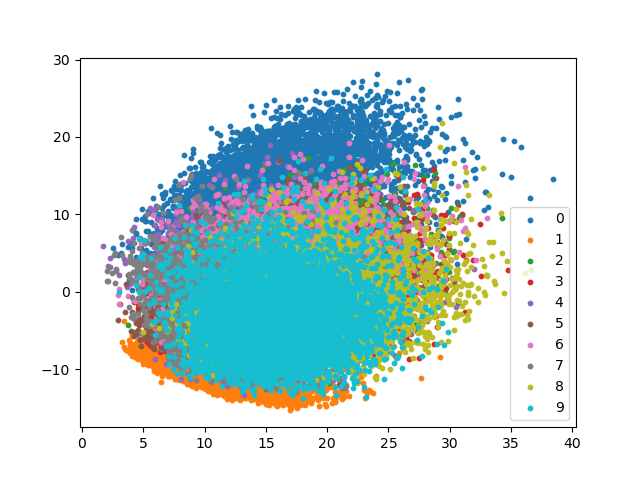
\includegraphics{hw4_q1}
	\caption{PCA Projection of MNIST Data}
\end{figure}

Overall, it did a good job at distinguishing 0 and 1, but other numbers were not very well differentiated. 


\bigskip

%------------------------------------------------

\newpage
\section{Multi-armed Bandits}
For MLP, \& the best optimizer was Adagrad with $\eta$ value of 0.01 without overfitting. 

%two plots, loss and projection 
\graphicspath{{/media/kimsh96453/SANDISK 128/23 Spring/CSCI5525/Homeworks/HW5/hw5_code_templates}}
\begin{figure}[h!]
	\centering
	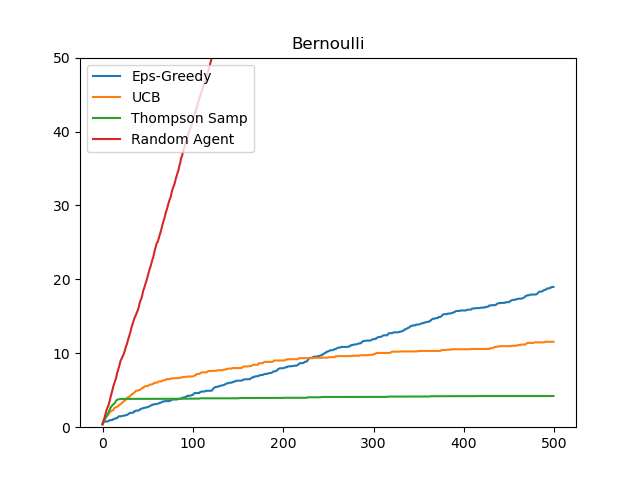
\includegraphics[scale=0.7]{hw5_2_Bernoulli}
	\caption{Autoencoder Training Loss by Epochs}
	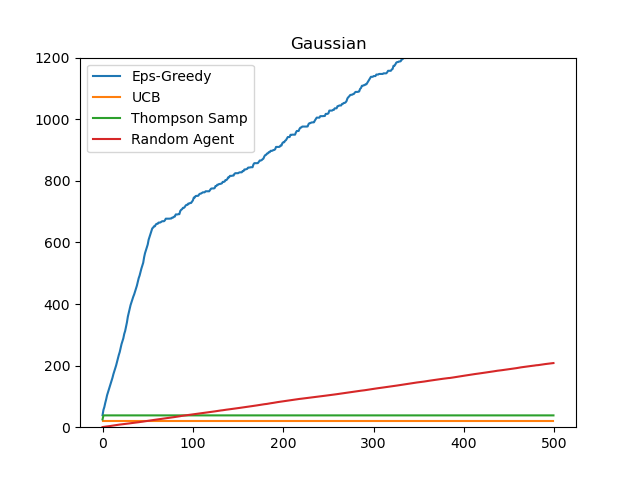
\includegraphics[scale=0.7]{hw5_2_Gaussian}
	\caption{Autoencoder Projection of 1000 Data Points}
	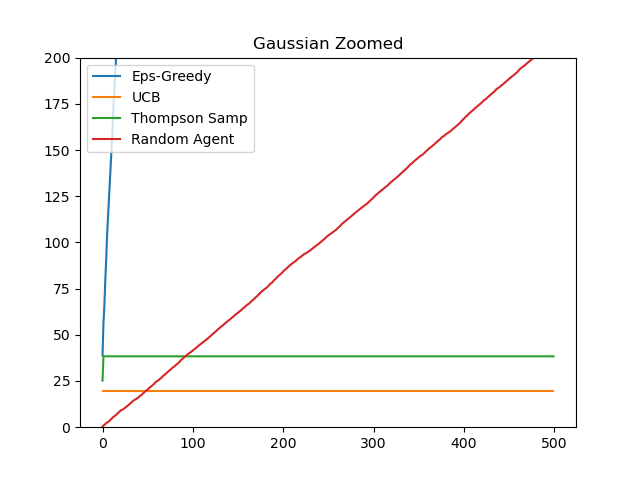
\includegraphics[scale=0.7]{hw5_2_Gaussian Zoomed}
\end{figure}

It was even more effective than PCA in distinguishing numbers, especially that are not 0 or 1. It did far better job than PCA for 0 and 1. It is also interesting that numbers are layered vertically. We can see 0, 6, 2 on upper side, 3, and 8 for middle, and 1, 9, 4, and 5 on the lower side. 

\bigskip



%------------------------------------------------

\end{document}
